% !TEX TS-program = pdflatex
% !TEX encoding = UTF-8 Unicode

% This is a simple template for a LaTeX document using the "article" class.
% See "book", "report", "letter" for other types of document.

\documentclass[11pt]{article} % use larger type; default would be 10pt

\usepackage[utf8]{inputenc} % set input encoding (not needed with XeLaTeX)

%%% Examples of Article customizations
% These packages are optional, depending whether you want the features they provide.
% See the LaTeX Companion or other references for full information.

%%% PAGE DIMENSIONS
\usepackage{geometry} % to change the page dimensions
\geometry{a4paper} % or letterpaper (US) or a5paper or....
% \geometry{margin=2in} % for example, change the margins to 2 inches all round
% \geometry{landscape} % set up the page for landscape
%   read geometry.pdf for detailed page layout information

\usepackage{graphicx} % support the \includegraphics command and options

% \usepackage[parfill]{parskip} % Activate to begin paragraphs with an empty line rather than an indent

%%% PACKAGES
\usepackage{booktabs} % for much better looking tables
\usepackage{array} % for better arrays (eg matrices) in maths
\usepackage{paralist} % very flexible & customisable lists (eg. enumerate/itemize, etc.)
\usepackage{verbatim} % adds environment for commenting out blocks of text & for better verbatim
\usepackage{subfig} % make it possible to include more than one captioned figure/table in a single float
% These packages are all incorporated in the memoir class to one degree or another...
\usepackage{pdfpages}
\usepackage{amsmath,mathtools,amsfonts}
\usepackage{bm}
\usepackage{float}
\usepackage{listings}\usepackage{color}

\definecolor{mygreen}{rgb}{0,0.6,0}
\definecolor{mygray}{rgb}{0.5,0.5,0.5}
\definecolor{mymauve}{rgb}{0.58,0,0.82}

\lstset{ 
	backgroundcolor=\color{white},   % choose the background color; you must add \usepackage{color} or \usepackage{xcolor}; should come as last argument
	basicstyle=\footnotesize,        % the size of the fonts that are used for the code
	breakatwhitespace=false,         % sets if automatic breaks should only happen at whitespace
	breaklines=true,                 % sets automatic line breaking
	captionpos=b,                    % sets the caption-position to bottom
	commentstyle=\color{mygreen},    % comment style
	deletekeywords={...},            % if you want to delete keywords from the given language
	escapeinside={\%*}{*)},          % if you want to add LaTeX within your code
	extendedchars=true,              % lets you use non-ASCII characters; for 8-bits encodings only, does not work with UTF-8
	firstnumber=001,                % start line enumeration with line 1000
	frame=single,	                   % adds a frame around the code
	keepspaces=true,                 % keeps spaces in text, useful for keeping indentation of code (possibly needs columns=flexible)
	keywordstyle=\color{blue},       % keyword style
	language=Octave,                 % the language of the code
	morekeywords={*,...},            % if you want to add more keywords to the set
	numbers=left,                    % where to put the line-numbers; possible values are (none, left, right)
	numbersep=5pt,                   % how far the line-numbers are from the code
	numberstyle=\tiny\color{mygray}, % the style that is used for the line-numbers
	rulecolor=\color{black},         % if not set, the frame-color may be changed on line-breaks within not-black text (e.g. comments (green here))
	showspaces=false,                % show spaces everywhere adding particular underscores; it overrides 'showstringspaces'
	showstringspaces=false,          % underline spaces within strings only
	showtabs=false,                  % show tabs within strings adding particular underscores
	stepnumber=2,                    % the step between two line-numbers. If it's 1, each line will be numbered
	stringstyle=\color{mymauve},     % string literal style
	tabsize=2,	                   % sets default tabsize to 2 spaces
	title=\lstname                   % show the filename of files included with \lstinputlisting; also try caption instead of title
}

%%% HEADERS & FOOTERS
\usepackage{fancyhdr} % This should be set AFTER setting up the page geometry
\pagestyle{fancy} % options: empty , plain , fancy
\renewcommand{\headrulewidth}{1pt} % customise the layout...
\lhead{Jesse Sheehan (53366509)}\chead{}\rhead{Will Cowper (81163265)}
\lfoot{}\cfoot{\thepage}\rfoot{}

%%% SECTION TITLE APPEARANCE
%\usepackage{sectsty}
%\allsectionsfont{\sffamily\mdseries\upshape} % (See the fntguide.pdf for font help)
% (This matches ConTeXt defaults)

%%% END Article customizations
\makeatletter
\renewcommand*\env@matrix[1][*\c@MaxMatrixCols c]{%
  \hskip -\arraycolsep
  \let\@ifnextchar\new@ifnextchar
  \array{#1}}
\makeatother

\newenvironment{sysmatrix}[1]
 {\left(\begin{array}{@{}#1@{}}}
 {\end{array}\right)}
\newcommand{\ro}[1]{%
  \xrightarrow{\mathmakebox[\rowidth]{#1}}%
}
\newlength{\rowidth}% row operation width
\AtBeginDocument{\setlength{\rowidth}{3em}}

\title{COSC364 RIPv2 Assignment}
\date{\today}
\author{Jesse Sheehan (53366509)\\ Will Cowper (81163265)}

\begin{document}

\maketitle

\tableofcontents

\newpage

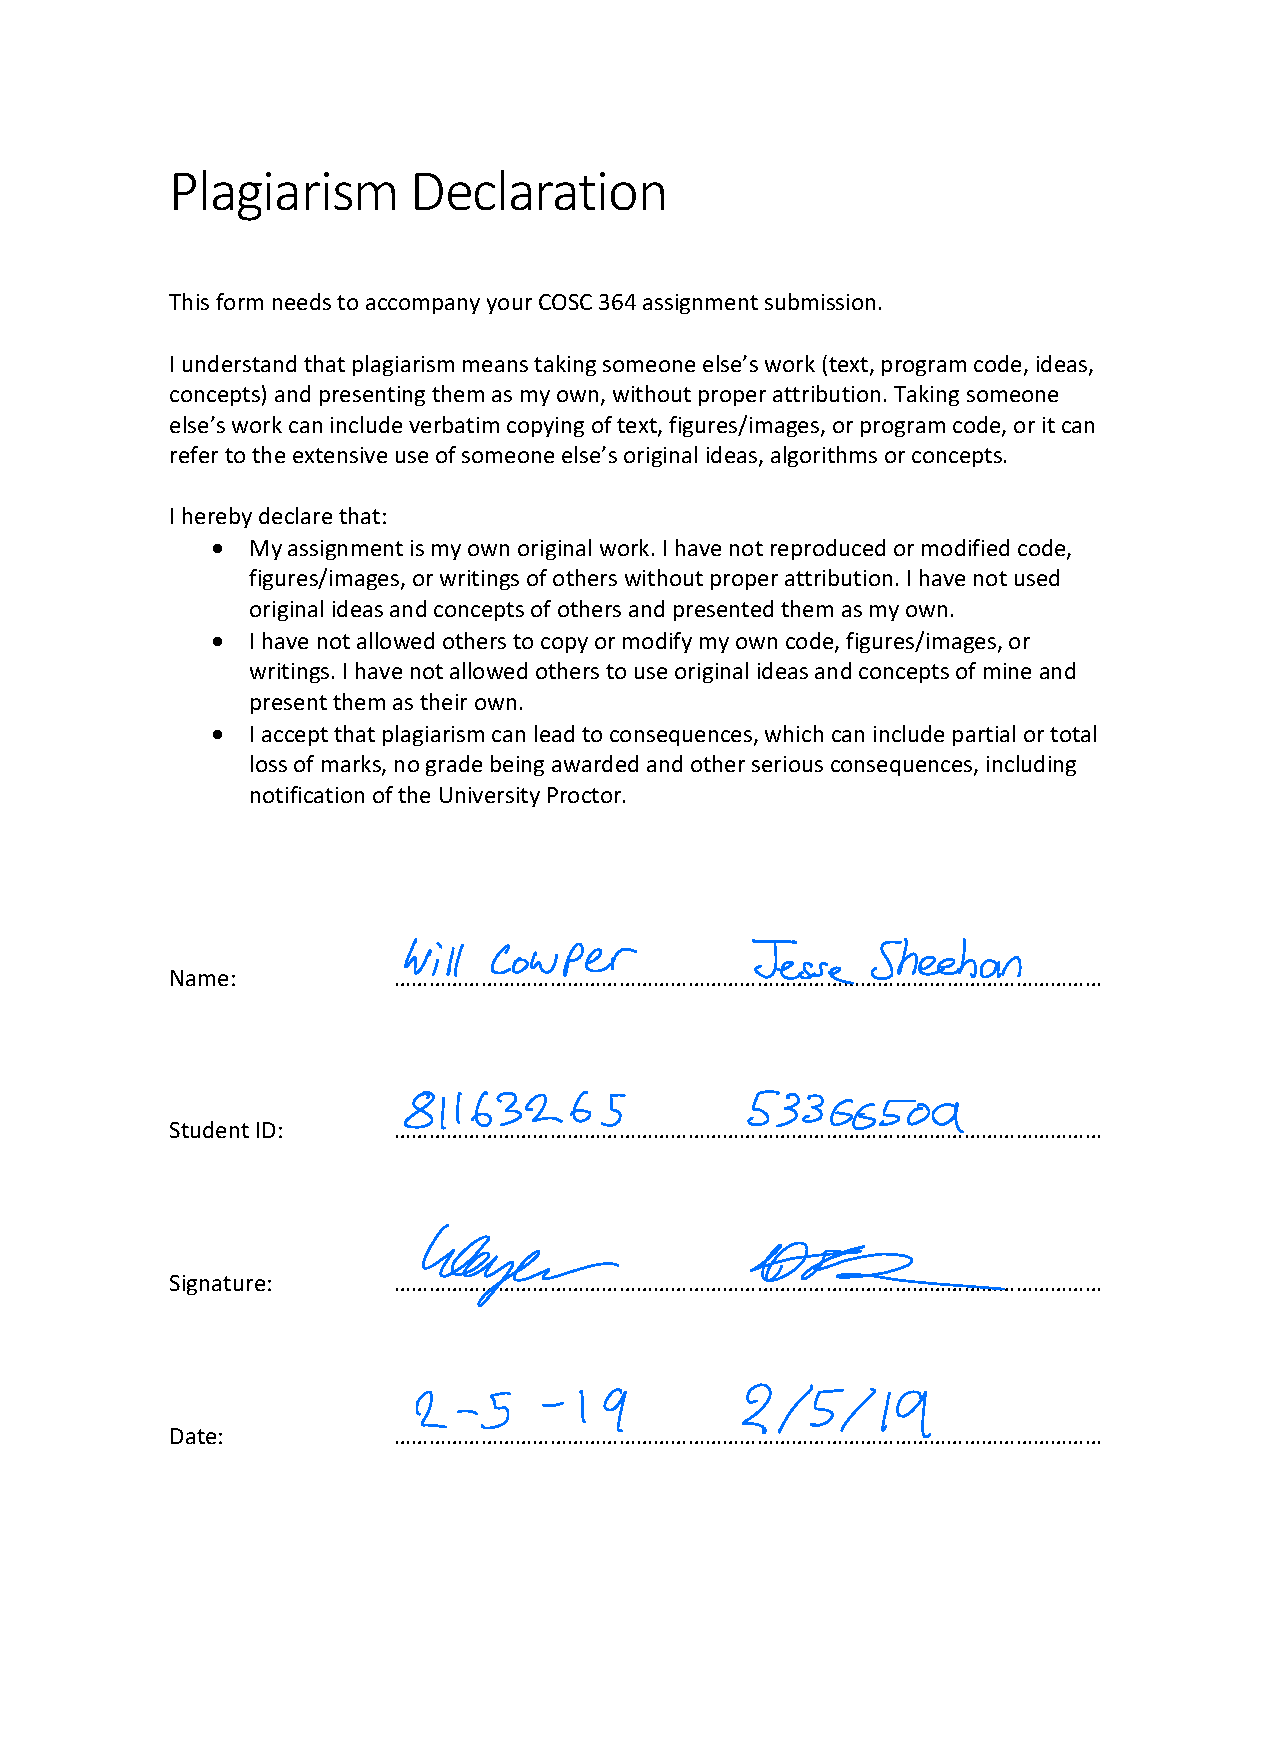
\includepdf[pages=1]{includes/plagiarism.pdf}

\section{Questions} \label{questions}

The configuration files of the example network can be found in sections \ref{figure1-start} to \ref{figure1-end}. The following questions have been answered:

\subsection{Contribution}
The contribution toward the entire project was an even split. We both felt as though the work we had contributed was worth 50\% each.

\subsection{Reflection} \label{reflection}

% Which aspects of your overall program do you consider to be particularly well done?
Some of the smaller modules in our codebase have been implemented quite well. For example, the Timer and Bencode modules have a very focused purpose and were discrete enough to be able to be doctested.
We found that making use of recursion in the Bencode module reduced the complexity that would have otherwise occurred.
The Timer module has many features that we didn't end up using but could be useful in the future if we decided to continue developing this project.
We also had a clean user-interface (see figure\ \ref{fig:interface}) that clearly displays the current routing table and some other information about the router.
Our protocol adds a CRC32 checksum to the data being sent, this is checked when the packet is received and dropped if it is incorrect. This protects our routers from receiving garbled packets.

\begin{figure}[H]
	\centering
	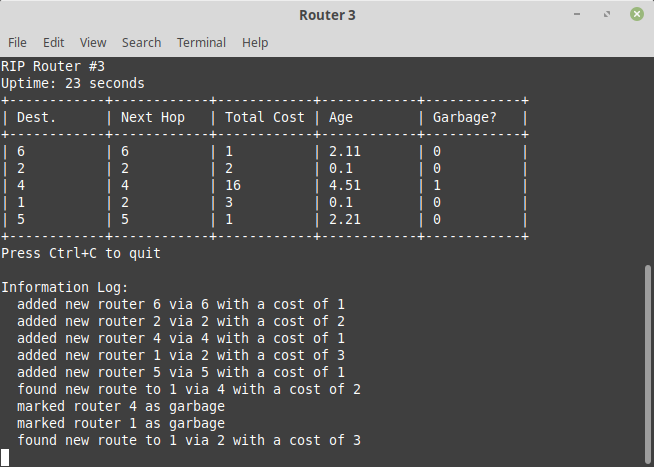
\includegraphics[width=0.8\textwidth]{includes/images/interface}
	\caption{The user interface of our router.}
	\label{fig:interface}
\end{figure}

% Which aspects of your overall program could be improved?
The overall system design could be improved.
We rewrote some modules several times in order to get it to feel as though it would be easy to work with.
We would also spend more time planning the project and understanding the exact steps required to implement the specification.
Our current solution only receives at most 4096 bytes of data when reading a packet, this means that we can only send a maximum of 81 full router table entries in a packet. This would become an issue if we had a router with more than 80 directly connected neighbors as we don't honour the RIP specification of limiting packets to a of maximum 25 entries. This could be overcome by fragmenting the entries and sending multiple packets with these entries.


\subsection{Event Processing} \label{event_processing}

% How have you ensured the atomicity of event processing?
Our entire program is based around a main loop that waits for incoming packets and if it doesn't receive any, it will do other things, such as updating the timers, updating the routing table, rendering the screen, etc. We use lists to ensure that our incoming packets are serviced in the order in which they arrive. When packets are processed, they may trigger updates to the routers neighbors. These updates are serviced after the periodic updates have finished being received. Once these updates have been sent to its neighbors, the router simply waits for more information to arrive.

In order to ensure the atomicity of events in our program we have made use of timer-driven functions and their timers in such a way that they do not  interrupt other events. Our entire program is single-threaded so we don't need to worry about interruptions from other parts of the program.


\subsection{Testing} \label{testing}

Many of the smaller functions in the project were discrete enough that we could use doctests on them.

Once we had most of the program working we had to create test configuration files for entire networks. We found this process to be very tedious and so, wrote a program to generate these files for us (see section \ref{generatenet}). Our testing became much easier after this as we didn't have to manually write these configuration files.

When testing an entire network, we would manually calculate the best routes by hand using the Bellman-Ford algorithm. We would then run the program and check that the routing table for each router converged to what we expected. We also tested our hypotheses for when an individual router was brought down using the same method. This would quite often reveal issues or bugs in our implementation that we could fix.\\

\noindent Given the "six-node" network (figure\ \ref{fig:sixnode}) below, the following tests were performed:

\begin{figure}[H]
	\centering
	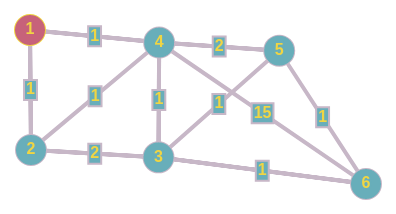
\includegraphics[width=0.8\textwidth]{includes/images/six-node}
	\caption{The "six-node" network as described in sections \ref{six-node-start} to \ref{six-node-end}.}
	\label{fig:sixnode}
\end{figure}

\begin{itemize}
\item \textbf{Configuration testing} - We created many configuration files for testing our config module. Some configuration files were well-formed and some were not. This allowed us to make sure that our config module worked as expected. For example, an empty config file would generate an error by our config parser. Another example, a config file with missing or invalid data.
\item \textbf{Brief outage} - Bringing a router down and then back up before the deletion process begins. We expected all routes using that router as a next hop would increase the age of the of their routing table entry but there would be no other change in the route entry or triggered updates/etc.
\item \textbf{Longer outage} - Bringing a router down and then waiting to bring the router back up after the deletion process begins but before it is purged from the other router's routing tables. We expected route poisoning to propogate through the network and routes to reconverge. When the router comes back up we expect all router table costs to return to their initial converged state. There is no guarantee that the next-hops will be the same. For example, if there are two or more routes with the same total cost to a common destination. In figure\ \ref{fig:sixnode} this can be seen at R2 which can reach R3 directly with a cost of 2 or through R1 with a cost of 2.
\item \textbf{Prolonged outage} - Bringing a router down and waiting for it to be purged from all routing tables. We expected the same behaviour as for the previous case with the route poisoning and reconvergence, as well as eventual purging of the downed router. When the router is brought back up, the router should be rediscovered by its neighbors and propogated by periodic updates. The network should converge to a state similar to the initial converged state (the route costs should be the same, but the next hops may be different).
\item \textbf{Multiple outages} - The previously described outage tests were performed again but by bringing down multiple routers at the same time instead. We expect the same correct behaviour (but obviously more widespread in some cases). For example, in the case of a router having all its directly connected neighbors brought offline, we would expect the routing table to be empty. Another example, all routers except R4 and R6 are brought down, this forces R4 and R6 to reach each other via the direct link with a cost of 15.
\item \textbf{Router significance} - Bringing down a router which isn't a next-hop router except for its directly neighbors (R6 in figure\ \ref{fig:sixnode}) We expect no reconvergence to take place. Comparing this behaviour with a router that is used by many routes, we would expect a great deal of reconvergence to take place by all routers whose routes use this router in their paths (R4 in figure\ \ref{fig:sixnode} has many neighbors that can be reached at low cost).
\end{itemize}

\noindent Often these tests would fail but we iterated on our source code and fixed the issues. Ultimately, we believe we have a bug-free implementation of the RIP protocol as described in the project specification.

\newpage
\section{Appendices}

\subsection{Source Code}

\subsubsection{src/\_\_main\_\_.py}
\lstinputlisting[language=Python]{../src/__main__.py}

\subsubsection{src/bencode.py}
\lstinputlisting[language=Python]{../src/bencode.py}

\subsubsection{src/config.py}
\lstinputlisting[language=Python]{../src/config.py}

\subsubsection{src/protocol.py}
\lstinputlisting[language=Python]{../src/protocol.py}

\subsubsection{src/routing\_table\_entry.py}
\lstinputlisting[language=Python]{../src/routing_table_entry.py}

\subsubsection{src/routing\_table.py}
\lstinputlisting[language=Python]{../src/routing_table.py}

\subsubsection{src/server.py}
\lstinputlisting[language=Python]{../src/server.py}

\subsubsection{src/timer.py}
\lstinputlisting[language=Python]{../src/timer.py}

\subsubsection{src/utils.py}
\lstinputlisting[language=Python]{../src/utils.py}

\newpage
\subsection{Configuration Files}

\subsubsection{configs/networks/figure1/1.conf} \label{figure1-start}
\lstinputlisting{../configs/networks/figure1/1.conf}

\subsubsection{configs/networks/figure1/2.conf}
\lstinputlisting{../configs/networks/figure1/2.conf}

\subsubsection{configs/networks/figure1/3.conf}
\lstinputlisting{../configs/networks/figure1/3.conf}

\subsubsection{configs/networks/figure1/4.conf}
\lstinputlisting{../configs/networks/figure1/4.conf}

\subsubsection{configs/networks/figure1/5.conf}
\lstinputlisting{../configs/networks/figure1/5.conf}

\subsubsection{configs/networks/figure1/6.conf}
\lstinputlisting{../configs/networks/figure1/6.conf}

\subsubsection{configs/networks/figure1/7.conf} \label{figure1-end}
\lstinputlisting{../configs/networks/figure1/7.conf}

\subsubsection{configs/networks/six-node/01.conf} \label{six-node-start}
\lstinputlisting{../configs/networks/six-node/01.conf}

\subsubsection{configs/networks/six-node/02.conf}
\lstinputlisting{../configs/networks/six-node/02.conf}

\subsubsection{configs/networks/six-node/03.conf}
\lstinputlisting{../configs/networks/six-node/03.conf}

\subsubsection{configs/networks/six-node/04.conf}
\lstinputlisting{../configs/networks/six-node/04.conf}

\subsubsection{configs/networks/six-node/05.conf}
\lstinputlisting{../configs/networks/six-node/05.conf}

\subsubsection{configs/networks/six-node/06.conf} \label{six-node-end}
\lstinputlisting{../configs/networks/six-node/06.conf}

\newpage
\subsection{Other Files}

\subsubsection{tools/generate\_network.py} \label{generatenet}
The following file will interactively prompt the user for information about a network. It will then create all the necessary configuration files for the network to run.
\lstinputlisting[language=Python]{../tools/generate_network.py}

\end{document}
